\documentclass[twoside]{article}

\usepackage{ustj}
\usepackage{cancel}
\usepackage{pdflscape}

\usepackage{tikz}
\newcommand{\bit}[1]{%
  \tikz[baseline=(char.base)]{%
    \node[shape=rectangle, draw, rounded corners=1pt, inner sep=1pt, minimum width=6pt, minimum height=6pt] (char) {#1};
  }%
}

\setcounter{tocdepth}{2}

\addbibresource{mss.bib}

\newcommand{\authorname}{Brian Klatt \patp{ticlys-monlun}, N. E. Davis \patp{lagrev-nocfep}}
\newcommand{\affiliation}{Zorp Corp}

%  Make first page footer:
\fancypagestyle{firststyle}{%
\fancyhf{}% Clear header/footer
\fancyhead{}
\fancyfoot[L]{{\footnotesize
              %% We toggle between these:
              % Manuscript submitted for review.\\
              {\it Urbit Systems Technical Journal} III:1 (2026):  83–101. \\
              % ~ \\
              Address author correspondence to \patp{lagrev-nocfep}.
              }}
}
%  Arrange subsequent pages:
\fancyhf{}
\fancyhead[LE]{{\urbitfont Urbit Systems Technical Journal}}
\fancyhead[RO]{Noun Serialization}
\fancyfoot[LE,RO]{\thepage}

%%MANUSCRIPT
\title{Noun Serialization}
\author{Brian Klatt \patp{ticlys-monlun}, \\ N. E. Davis \patp{lagrev-nocfep}* \\ \affiliation}
\date{}

\begin{document}

\maketitle
\thispagestyle{firststyle}

\begin{abstract}
Noun serialization is commonly used for Nock communication, both between instances like Urbit ships and with the runtime and the Unix host operating system.  This article describes the principal convention for representing a noun in compressed form as a byte array and its runtime affordance.
\end{abstract}

\renewcommand{\thefootnote}{\fnsymbol{footnote}}
\setcounter{footnote}{0}
\footnotetext[1]{\sloppy We gratefully acknowledge the original architect of \texttt{+jam} and \texttt{+cue}, \mbox{Curtis} Yarvin \patp{sorreg-namtyv}.  The earliest implementation, in \href{https://github.com/cgyarvin/urbit/blame/55f591594080d276fc446ceafa4afff092561613/watt/jam.watt}{\texttt{jam.watt}}, dates to \textasciitilde 2011.6.11; Yarvin has indicated that an earlier draft no longer survives.}
\renewcommand{\thefootnote}{\arabic{footnote}}
\setcounter{footnote}{0}

% We will adjust page numbering in final editing.
\pagenumbering{arabic}
\setcounter{page}{83}

\tableofcontents

\section{Introduction}

The Nock combinator calculus deals in nouns and does not know about bit encodings or memory layouts.  A Nock interpreter (runtime) must, however, deal with the practicalities.  In other words, there must be a way of writing down an abstract binary tree (consisting of cells/pairs and atoms) as an actual, physical array of bits in memory.  Every possible Nock noun can be represented as a finite sequence of bytes (an atom), and there are multiple ways to do so.\footnote{The converse is not true:  not every atom represents a valid deserialization or conversion from a graph encoding.}

A noun serialization strategy is rather like a Gödel numbering in that it systematically encodes a mathematical object (a noun) as a number (an atom).  Unlike Gödel numbering, which classically serially encodes the symbols of mathematical statements, noun serialization encodes a binary tree structure.\footnote{This also echoes the way that S-expressions are encoded in Lisp.}  Because a noun may be any atom---and atoms cannot have leading zeroes---both structure and value need to be unambiguously encoded and cannot be simply delimited (as by a \texttt{0} bit or similar).  Run-length serialization, with or without references, forms the basis of practical strategies to encode a noun as an atom.  This embodies a tradeoff between simplicity, size, and speed.  We describe this strategy and some pedagogical variants which afford insight to the process.  Likewise, deserialization is the inverse operation of converting a serialized atom back into the original noun, and must be unambiguously reversible.  Noun serialization is essential for Nock communication, both between Nock execution layers such as Vere and NockVM, and between the runtime and the host operating system.

\section{Na\"{i}ve Serialization}

A noun may be an atom or a cell, and so we first propose to label nodes by type, with \texttt{0} for atom and \texttt{1} for cell.

\begin{figure}[ht]
  \centering
  % ---------- left tree ----------
  \begin{subfigure}{\textwidth}
    \centering
    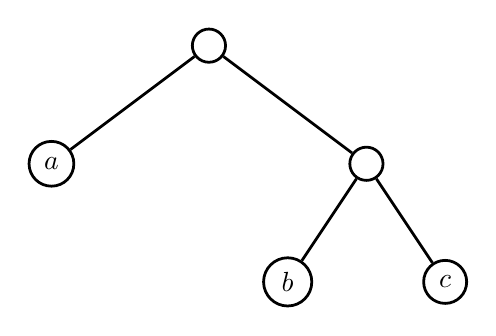
\begin{tikzpicture}[
        level 1/.style={sibling distance=40mm, line width=1pt},
        level 2/.style={sibling distance=20mm, line width=1pt},
        every node/.style={circle, draw, line width=1pt, minimum size=1.2em}
      ]
      \node {}
        child { node {$a$} }
        child { node {}
          child { node {$b$} }
          child { node {$c$} }
        };
    \end{tikzpicture}
  \end{subfigure}
  \\
  % ---------- right tree ----------
  \begin{subfigure}{\textwidth}
    \centering
    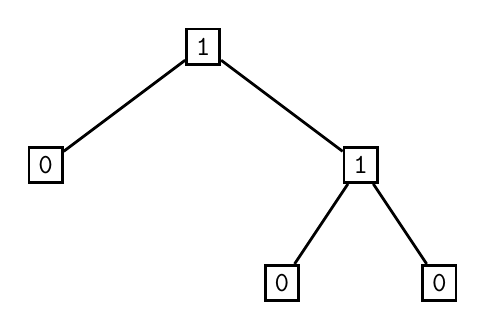
\begin{tikzpicture}[
        level 1/.style={sibling distance=40mm, line width=1pt},
        level 2/.style={sibling distance=20mm, line width=1pt},
        every node/.style={rectangle, draw, line width=1pt, minimum size=1.2em}
      ]
      \node {\texttt{1}}
        child { node {\texttt{0}} }
        child { node {\texttt{1}}
          child { node {\texttt{0}} }
          child { node {\texttt{0}} }
        };
    \end{tikzpicture}
  \end{subfigure}

  \caption{The noun \texttt{[a b c]} (the same as \texttt{[a [b c]]}) as a binary tree and its metadata labeling in the simplest scheme.}
  \label{fig:binary-tree}
\end{figure}

\noindent
The noun in Figure~\ref{fig:binary-tree} is represented as a binary tree, where each node is labeled with its type (atom or cell) and its value (if applicable).  To serialize this noun, we can perform a pre-order traversal of the tree, recording the type and value of each node.  The serialized form would be (in \textsc{lsb} order):

\begin{lstlisting}[style=listingcode]
c 0 b 0 1 a 0 1
\end{lstlisting}

\noindent
The issue, however, is that in decoding this bitstream we do not know where an atom value (such as \texttt{a}) ends.  After all, the point of serialization is to be able to deserialize the bitstream back into the original noun.  Thus we need a way to indicate the length of each atom.

\subsection{Atom Length Encoding}

Let's augment this scheme by providing length information for each atom.  One basic idea is to include a string of \texttt{0} bits as the least-significant bits (\textsc{lsb}) of the atom which indicates the length of the atom in bits.  Since the atom could be zero, we also delimit the length with a \texttt{1} bit.  (See Table~\ref{tab:atom-encodings} for examples.)

$$
a = a_{\ell-1} a_{\ell-2} \ldots a_{1} a_{0}
\xrightarrow[\textrm{encode}]{}
\bar{a} = a_{\ell-1} a_{\ell-2} \ldots a_{1} a_{0} \; \mathtt{1} \; \mathtt{0}^{n}
\textrm{,}
$$

\noindent
where $\bar{a}$ is the encoded atom $a$ and $a$ has length $\ell$ bits.\footnote{We will use the overbar notation $\bar{a}$ throughout to notionally indicate the encoded form of $a$, regardless of the method used.}  This is a unary run-length encoding (\textsc{rle}) using zeros.\footnote{Zero is something of a ``special case'':  it has no length and leading zeros are trimmed, so its encoding consists only of the delimiter, \texttt{0b1}.}

\begin{table}[ht]
\centering
\caption{Example atom encodings with length information appended as trailing zeros (unnamed encoding).}
\label{tab:atom-encodings}
\begin{tabular}{ l l r }
  \textbf{Atom} $\bm{a}$ & \textbf{Length (bits)} & \multicolumn{1}{l}{\textbf{Encoded Form} $\bm{\bar{a}}$} \\
  \hline
  \texttt{0b0} & 1 & \texttt{0b1} \\
  \texttt{0b1} & 1 & \texttt{0b110} \\
  \texttt{0b10} & 2 & \texttt{0b10100} \\
  \texttt{0b11} & 2 & \texttt{0b11100} \\
  \texttt{0b101} & 3 & \texttt{0b1011000} \\
  \texttt{0b111} & 3 & \texttt{0b1111000} \\
  \texttt{0x70} & 7 & \texttt{0b111000010000000} \\
  \texttt{0xff} & 8 & \texttt{0b11111111100000000} \\
  \texttt{0x1234} & 13 & \texttt{0b1001000110100} \\
  & & \texttt{↳10000000000000} \\
\end{tabular}
\end{table}

\noindent
We can make one further optimization:  since the most significant bit (\textsc{msb}) of the atom is always \texttt{1} except in the case of zero (which is \texttt{0b1} with the leading zero trimmed), we can omit it from the encoded form.  This saves one bit for every non-zero atom.  Let's call this scheme \texttt{+fat} encoding.  (See Table~\ref{tab:fat-encodings} for examples.)

\paragraph*{\texttt{+fat} Serialization Algorithm}

\begin{itemize}
\item  \textbf{Encode}.  Write\footnote{We always say this from the \textsc{lsb}, so from the right as written on the page.} $\ell$ bits of \texttt{0}, where $\ell$ is the length of $a$ in unary, followed by \texttt{1}.  The next $\ell$ bits are the atom $a$ in binary without the leading \texttt{1}.
\item  \textbf{Decode}.  Read the unary length $\ell$ by counting \texttt{0} bits until the first \texttt{1} bit.  Read the next $\ell$ bits to get the atom $a$ without the leading \texttt{1}.  Prepend a \texttt{1} bit to $a$ unless $\ell$ is zero, in which case the atom is zero.
\end{itemize}

\begin{table}[ht]
\centering
\caption{Example atom encodings (\texttt{+fat} encoding).  Elided digits are shown in light gray for clarity.}
\label{tab:fat-encodings}
\begin{tabular}{ l l r }
  \textbf{Atom} $\bm{a}$ & \textbf{Length (bits)} & \multicolumn{1}{l}{\textbf{Encoded Form} $\bm{\bar{a}}$} \\
  \hline
  \texttt{0b0} & 1 & \texttt{0b1} \\
  \texttt{0b1} & 1 & \texttt{0b\textcolor{lightgray}{1}10} \\
  \texttt{0b10} & 2 & \texttt{0b\textcolor{lightgray}{10}100} \\
  \texttt{0b11} & 2 & \texttt{0b\textcolor{lightgray}{1}1100} \\
  \texttt{0b101} & 3 & \texttt{0b\textcolor{lightgray}{10}11000} \\
  \texttt{0b111} & 3 & \texttt{0b\textcolor{lightgray}{1}111000} \\
  \texttt{0x70} & 7 & \texttt{0b\textcolor{lightgray}{1}11000010000000} \\
  \texttt{0xff} & 8 & \texttt{0b\textcolor{lightgray}{1}1111111100000000} \\
  \texttt{0x1234} & 13 & \texttt{0b\textcolor{lightgray}{100}1000110100} \\
  & & \texttt{↳10000000000000} \\
\end{tabular}
\end{table}

The primary problem with the \texttt{+fat} scheme is that the encoding of an atom is about twice the bit length of the original atom.  The next optimization is to use the bit length of the unary bit length, which is logarithmic in the bit length.

$$
a =
\underbrace{a_{\ell-1} a_{\ell-2} \ldots a_{1} a_{0}}
_{\textstyle \mathrlap{\kern-0.25em\ell =
\underbrace{\ell_{h-1} \ell_{h-2} \ldots \ell_{1} \ell_{0}}
_{\textstyle h}}}
$$

\begin{align*}
a = & a_{\ell-1} a_{\ell-2} \ldots a_{1} a_{0}
\xrightarrow[\textrm{\texttt{+mat} encode}]{}
\\
\bar{a} = &
\underbrace{a_{\ell-1} a_{\ell-2} \ldots a_{1} a_{0}}
_{\ell}
\underbrace{\ell_{h-2} \ell_{h-1} \ldots \ell_{1} \ell_{0}}
_{h-1}
\mathtt{1}
\underbrace{\mathtt{0} \ldots \mathtt{0}}
_{h}
\textrm{,}
\end{align*}

\noindent
where $\ell$ is the bit length of $a$ and $h$ is the ``hyper bit length'' of $a$.  This yields a bit length encoding of $1+2\log_2(\ell)$ bits rather than $2\ell$ bits.  This scheme is called \lstinline[style=inlinecode]{+mat} encoding, and it is currently in use as an internal auxiliary format for other serializations.

\paragraph*{\texttt{+mat} Serialization Algorithm}

\begin{itemize}
\item  \textbf{Encode}.  Write the number $h$ of \texttt{0} bits in unary, followed a leading \texttt{1} and then $h-1$ bits for the low bits of $\ell$.  The next $\ell$ bits are the atom $a$ in binary.
\item  \textbf{Decode}.  Read the unary length of the length $h$ by counting \texttt{0} bits (from the \textsc{lsb}/right) until the first \texttt{1} bit.  Read the next $h-1$ bits to get $\ell-1$, the bit length of the atom.  Finally, read the next $\ell$ bits (adding the leading \texttt{1}) to get the atom $a$.
\end{itemize}

Some worked examples of \texttt{+mat} encoding are included in Table~\ref{tab:mat-encodings}.

The reference implementation of \texttt{+mat} encoding in Hoon is as follows:

\begin{lstlisting}[style=listingcode]
++  mat
  ~/  %mat
  |=  a=@
  ^-  [p=@ q=@]
  ?:  =(0 a)
    [1 1]
  =+  b=(met 0 a)
  =+  c=(met 0 b)
  :-  (add (add c c) b)
  (cat 0 (bex c) (mix (end [0 (dec c)] b)
   ↳                  (lsh [0 (dec c)] a)))
\end{lstlisting}

\begin{landscape}
\begin{table}[ht]
\centering
\caption{Example atom encodings (\texttt{+mat} encoding).  The encoded form is the same result as \texttt{q:(mat a)} in Hoon.}
\label{tab:mat-encodings}
\begin{tabular}{ r c r l r }
  \multicolumn{1}{l}{\textbf{Atom}} $\bm{a}$ & \textbf{Length (bits)} & \multicolumn{2}{c}{\hspace{2cm}\textbf{Mathematics}} & \multicolumn{1}{c}{\textbf{Encoded Form} $\bm{\bar{a}}$} \\
  \hline
  \texttt{0b0} & $\ell = 1$ & $\underbrace{\cancel{{a_{\ell-1}}}\ldots\cancel{a_{0}}}_{\ell=0}$&$\mathtt{1}\underbrace{\cancel{\mathtt{0}}\ldots\cancel{\mathtt{0}}}_{h=0}$ & \texttt{0b1} \\
  \texttt{0b1} & $\ell = 1$ & $\underbrace{\mathtt{1}}_{\ell=1}\underbrace{\cancel{{\ell_{h-2}}}\ldots\cancel{\ell_{0}}}_{h-1=0}$&$\mathtt{1}\underbrace{\mathtt{0}}_{h=1}$ & \texttt{0b110} \\
  \texttt{0b10} & $\ell = 2$ & $\underbrace{\mathtt{10}}_{a=2}\underbrace{\mathtt{0}}_{\textrm{low bits of }\ell}$&$\mathtt{1}\underbrace{\mathtt{00}}_{h=2}$ & \texttt{0b100100} \\
  \texttt{0b11} & $\ell = 2$ & $\underbrace{\mathtt{11}}_{a=3}\underbrace{\mathtt{0}}_{\textrm{low bits of }\ell}$&$\mathtt{1}\underbrace{\mathtt{00}}_{h=2}$ & \texttt{0b110100} \\
  \texttt{0b100} & $\ell = 3$ & $\underbrace{\mathtt{100}}_{a=4}\underbrace{\mathtt{1}}_{\textrm{low bits of }\ell}$&$\mathtt{1}\underbrace{\mathtt{00}}_{h=2}$ & \texttt{0b1001100} \\
  \texttt{0b101} & $\ell = 3$ & $\underbrace{\mathtt{101}}_{a=5}\underbrace{\mathtt{1}}_{\textrm{low bits of }\ell}$&$\mathtt{1}\underbrace{\mathtt{00}}_{h=2}$ & \texttt{0b1011100} \\
  \texttt{0b1111} & $\ell = 4$ & $\underbrace{\mathtt{1111}}_{a=15}\underbrace{\mathtt{00}}_{\textrm{low bits of }\ell}$&$\mathtt{1}\underbrace{\mathtt{000}}_{h=3}$ & \texttt{0b1111001000} \\
  \texttt{0x70} & $\ell = 7$ & $\underbrace{\mathtt{1110000}}_{a=112}\underbrace{\mathtt{11}}_{\textrm{low bits of }\ell}$&$\mathtt{1}\underbrace{\mathtt{000}}_{h=3}$ & \texttt{0b1110000111000} \\
  \texttt{0x1234} & $\ell = 13$ & $\underbrace{\mathtt{1001000110100}}_{a=4660}\underbrace{\mathtt{101}}_{\textrm{low bits of }\ell}$&$\mathtt{1}\underbrace{\mathtt{0000}}_{h=4}$ & \texttt{0b100100011010010110000} \\
\end{tabular}
\end{table}
\end{landscape}

\sloppy
With \texttt{+mat} encoding in hand, we can produce a proper \mbox{serialization} scheme for nouns by combining the type bit with the encoded atom or recursively encoding cells.  We call this scheme \texttt{+gel} encoding.

As before, we use \texttt{0} for atom and \texttt{1} for cell.  If the noun is an atom, we follow the type bit with the \texttt{+mat} encoding of the atom.  If the noun is a cell, we follow the type bit with the \texttt{+gel} encoding of the head and then the \texttt{+gel} encoding of the tail.

Consider the noun \texttt{[a [b c]]} (= \texttt{[a b c]}), represented as a binary tree in Figure~\ref{fig:binary-tree-example}.  Reading across in a depth-first traversal, we produce an encoding order:

\begin{lstlisting}[style=listingblock]
(mat 1)(0)(mat 0)(0)(1)(mat 4)(0)(1)
\end{lstlisting}

\noindent
We already have the \texttt{+mat} encodings from Table~\ref{tab:mat-encodings}; substituting these in yields:

\begin{lstlisting}[style=listingblock]
[110](0)[1](0)(1)[1001100](0)(1)
0b110.0.1.0.1.1001100.0.1
0b1100101100110001
\end{lstlisting}

\begin{figure}[ht]
  \centering
  % ---------- left tree ----------
  \begin{subfigure}{\textwidth}
    \centering
    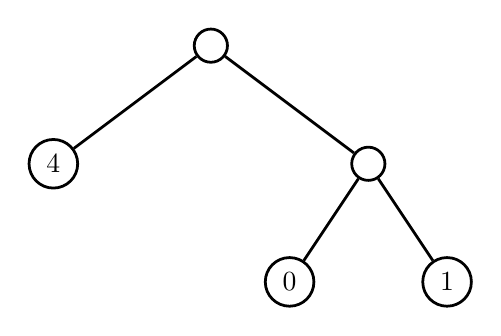
\begin{tikzpicture}[
        level 1/.style={sibling distance=40mm, line width=1pt},
        level 2/.style={sibling distance=20mm, line width=1pt},
        every node/.style={circle, draw, line width=1pt, minimum size=1.2em}
      ]
      \node {}
        child { node {4} }
        child { node {}
          child { node {0} }
          child { node {1} }
        };
    \end{tikzpicture}
  \end{subfigure}
  \\
  % ---------- right tree ----------
  \begin{subfigure}{\textwidth}
    \centering
    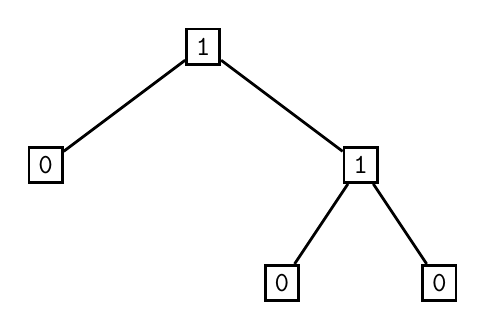
\begin{tikzpicture}[
        level 1/.style={sibling distance=40mm, line width=1pt},
        level 2/.style={sibling distance=20mm, line width=1pt},
        every node/.style={rectangle, draw, line width=1pt, minimum size=1.2em}
      ]
      \node {\texttt{1}}
        child { node {\texttt{0}} }
        child { node {\texttt{1}}
          child { node {\texttt{0}} }
          child { node {\texttt{0}} }
        };
    \end{tikzpicture}
  \end{subfigure}

  \caption{The noun \texttt{[4 0 1]} as a binary tree and its metadata labeling in the simplest scheme.  Compare Figure~\ref{fig:binary-tree}.}
  \label{fig:binary-tree-example}
\end{figure}

\paragraph*{\texttt{+gel} Serialization Algorithm}
\begin{itemize}
\item  \textbf{Encode}.
  \begin{itemize}
    \item  If the noun is an atom, write \texttt{0} followed by the \texttt{+mat} encoding of the atom.
    \item  If the noun is a cell, write \texttt{1} followed by the \texttt{+gel} encoding of the head and then the \texttt{+gel} encoding of the tail.
  \end{itemize}
\item  \textbf{Decode}.  Read the first bit.
  \begin{itemize}
    \item  If it is \texttt{0}, read the next bits as a \texttt{+mat} encoded atom.
    \item  If it is \texttt{1}, recursively read the next bits as the head and then the tail.
  \end{itemize}
\end{itemize}

\texttt{+gel} encoding is straightforward to read and write even by hand.  Worked examples are included in Table~\ref{tab:gel-encodings}.

\begin{table}[ht]
\centering
\caption{Example noun encodings (\texttt{+gel} encoding).  \texttt{.} dot delimits bit fields for readability.}
\label{tab:gel-encodings}
\begin{tabular}{ r r }
  \multicolumn{1}{l}{\textbf{Noun}} & \multicolumn{1}{l}{\textbf{Encoded Form}} \\
  \hline
  \texttt{0} & \texttt{0b0.1.0} \\
  \texttt{[0 0]} & \texttt{0b1.0.1.0.1} \\
  \texttt{[1 0]} & \texttt{0b1.0.110.0.1} \\
  \texttt{[2 1 0]} & \texttt{0b1.0.110.0.1.100100.0.1} \\
  \texttt{[[2 3] 1 0]} & \texttt{0b1.0.110.0.1.110100.0.100100.0.1.1} \\
\end{tabular}
\end{table}

\newpage
Our code implementation for \texttt{+gel} encoding is as follows:

\begin{lstlisting}[style=listingcode]
++  gel
  |=  a=*
  ^-  @
  =+  b=0
  =<  q
  |-  ^-  [p=@ q=@]
  ?:  ?=(@ a)
    =+  d=(mat a)
    [(add 1 p.d) (lsh 0 q.d)]
  =>  .(b (add 1 b))
  =+  d=$(a -.a)
  =+  e=$(a +.a, b (add b p.d))
  :-  (add 1 (add p.d p.e))
  (mix 1 (lsh [0 1] (cat 0 q.d q.e)))
\end{lstlisting}

\noindent
Decoding is left as an exercise to the interested reader.

\section{Practical Serialization}

Whatever the pedagogical advantages of \texttt{+gel}, the algorithm is still relatively verbose.  Nock-based operating functions have preferred in practice to use \texttt{+jam} encoding, which is a more compact run-length encoding with subtree deduplication.\footnote{Note the calculation of \patp{dozreg-toplud}, p.~57 of this issue, that an operational Arvo instance may have up to $1.66 \times 10^{21}$ nouns, greatly reduced by structural sharing.}  \texttt{+jam} improves the basic strategy by altering the \textsc{rle} algorithm slightly and supporting internal references for noun subtrees that have already been encoded.

\texttt{+jam} converts a noun into a buffer and deduplicates repeated subtrees.  It walks subtrees and encodes each in a way that allows for efficient storage and retrieval, while also permitting references to previously encoded values.  Basically, it takes \texttt{+gel} and adds a ``caching mode'' flag; instead of repeating subtrees, encode the index in the full jammed noun to where the current node's jammed subnoun was first written.  Thus the code changes from \texttt{0} for atom and \texttt{1} for cell to:

\begin{itemize}
  \item  \texttt{0} for atom.
  \item  \texttt{01} for cell.
  \item  \texttt{11} for cached node.
\end{itemize}

\begin{figure}[ht]
  \centering
  % ---------- left tree ----------
  \begin{subfigure}{\textwidth}
    \centering
    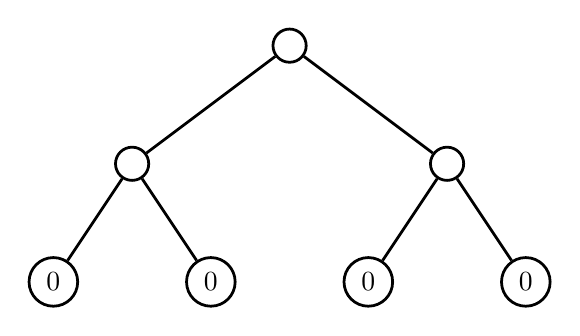
\begin{tikzpicture}[
        level 1/.style={sibling distance=40mm, line width=1pt},
        level 2/.style={sibling distance=20mm, line width=1pt},
        every node/.style={circle, draw, line width=1pt, minimum size=1.2em}
      ]
      \node {}
        child { node {}
          child { node {0} }
          child { node {0} }
        }
        child { node {}
          child { node {0} }
          child { node {0} }
        };
    \end{tikzpicture}
  \end{subfigure}
  \\
  % ---------- right tree ----------
  \begin{subfigure}{\textwidth}
    \centering
    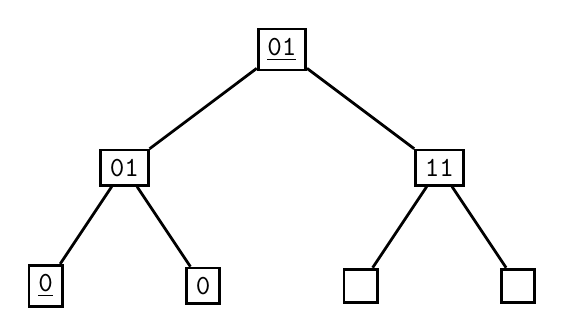
\begin{tikzpicture}[
        level 1/.style={sibling distance=40mm, line width=1pt},
        level 2/.style={sibling distance=20mm, line width=1pt},
        every node/.style={rectangle, draw, line width=1pt, minimum size=1.2em}
      ]
      \node {\underline{\texttt{01}}}
        child { node {\texttt{01}}
          child { node {\underline{\texttt{0}}} }
          child { node {\texttt{0}} }
        }
        child { node {\texttt{11}}
          child { node {} }
          child { node {} }
        };
    \end{tikzpicture}
  \end{subfigure}

  \caption{The noun \texttt{[[0 0] 0 0]} as a binary tree and its metadata labeling for the \texttt{+jam} scheme.}
  \label{fig:binary-tree-jam}
\end{figure}

Following the metadata labels given in Figure~\ref{fig:binary-tree-jam}, the encoding order for \texttt{[[0 0] 0 0]} is:

\begin{lstlisting}[style=listingblock]
(mat 2)(11)(mat 0)(0)(mat 0)((@$\underline{\mathtt{0}}$@))(01)((@$\underline{\mathtt{01}}$@))
0b100100.11.1.0.1.(@$\underline{\mathtt{0}}$@).01.(@$\underline{\mathtt{01}}$@)
0b1001001110100101
\end{lstlisting}

\noindent
The cached entry \texttt{(mat 2)} indicates that the cached subtree is a copy of the subtree located at tree address 2 in the overall jammed noun.

However, this bit of cleverness isn't the end:  \texttt{+jam} also decides \emph{when} to cache subtrees based on the size of the nouns involved.  For instance, \texttt{[3 3 3]} encodes as:

\begin{lstlisting}[style=listingblock]
(mat 3)(0)(mat 3)(0)(01)(mat 3)(0)(01)
0b110100.0.110100.0.01.110100.0.01
0b1101000110100001110100001
\end{lstlisting}

\noindent
wherein no caching is used.  When 3 is first encountered at index 2, 2 and 3 have the same bit lengths; since \texttt{(mat 2)} and \texttt{(mat 3)} are the same length, caching would not save any space and would add decoding overhead due to dereferencing.

In contrast, \texttt{[4 4 4]} encodes as:

\begin{lstlisting}[style=listingblock]
(mat 2)(11)(mat 2)(11)(01)(1001100)(0)(01)
0b100100.11.100100.11.01.1001100.0.01
0b1001001110010011011001100001
\end{lstlisting}

\noindent
where caching is used for the second and third occurrences of 4.  Here, 4 has bit length 3 which is greater than the bit length of 2 which is 2, and caching saves space overall in the jammed noun.

\paragraph*{\texttt{+jam} Serialization Algorithm}

\begin{itemize}
\item  \textbf{Encode}.
  \begin{itemize}
    \item  If the noun is an atom, write \texttt{0} followed by the \texttt{+mat} encoding of the atom.
    \item  If the noun is a cell, check if it has been previously encoded.
      \begin{itemize}
        \item  If it has, write \texttt{11} followed by the \texttt{+mat} encoding of the index where it was first encoded.
        \item  If it has not, write \texttt{01} followed by the \texttt{+jam} encoding of the head and then the \texttt{+jam} encoding of the tail.  Store the current index for future reference.
      \end{itemize}
  \end{itemize}
\item  \textbf{Decode}.  Read the first bit.
  \begin{itemize}
    \item  If it is \texttt{0}, read the next bits as a \texttt{+mat} encoded atom.
    \item  If it is \texttt{1}, read the next bit.
      \begin{itemize}
        \item  If it is \texttt{0}, recursively read the next bits as the head and then the tail.
        \item  If it is \texttt{1}, read the next bits as a \texttt{+mat} encoded index and retrieve the cached subtree.
      \end{itemize}
  \end{itemize}
\end{itemize}

Here is the reference implementation of \texttt{+jam} in Hoon:

\begin{lstlisting}[style=listingcode]
++  jam
  ~/  %jam
  |=  a=*
  ^-  @
  =+  b=0
  =+  m=`(map * @)`~
  =<  q
  |-  ^-  [p=@ q=@ r=(map * @)]
  =+  c=(~(get by m) a)
  ?~  c
    =>  .(m (~(put by m) a b))
    ?:  ?=(@ a)
      =+  d=(mat a)
      [(add 1 p.d) (lsh 0 q.d) m]
    =>  .(b (add 2 b))
    =+  d=$(a -.a)
    =+  e=$(a +.a, b (add b p.d), m r.d)
    :+  (add 2 (add p.d p.e))
      (mix 1 (lsh [0 2] (cat 0 q.d q.e)))
    r.e
  ?:  ?&(?=(@ a) (lte (met 0 a) (met 0 u.c)))
    =+  d=(mat a)
    [(add 1 p.d) (lsh 0 q.d) m]
  =+  d=(mat u.c)
  [(add 2 p.d) (mix 3 (lsh [0 2] q.d)) m]
\end{lstlisting}

\sloppy
A Python implementation of \texttt{+jam} is included in the \mbox{appendix}.

Here is the reference implementation of \texttt{+cue} in Hoon:

\begin{lstlisting}[style=listingcode]
++  cue
  ~/  %cue
  |=  a=@
  ^-  *
  =+  b=0
  =+  m=`(map @ *)`~
  =<  q
  |-  ^-  [p=@ q=* r=(map @ *)]
  ?:  =(0 (cut 0 [b 1] a))
    =+  c=(rub +(b) a)
    [+(p.c) q.c (~(put by m) b q.c)]
  =+  c=(add 2 b)
  ?:  =(0 (cut 0 [+(b) 1] a))
    =+  u=$(b c)
    =+  v=$(b (add p.u c), m r.u)
    =+  w=[q.u q.v]
    [(add 2 (add p.u p.v)) w (~(put by r.v) b w)]
  =+  d=(rub c a)
  [(add 2 p.d) (need (~(get by m) q.d)) m]
::  length decode
++  rub
  ~/  %rub
  |=  [a=@ b=@]
  ^-  [p=@ q=@]
  =+  ^=  c
      =+  [c=0 m=(met 0 b)]
      |-  ?<  (gth c m)
      ?.  =(0 (cut 0 [(add a c) 1] b))
        c
      $(c +(c))
  ?:  =(0 c)
    [1 0]
  =+  d=(add a +(c))
  =+  e=(add (bex (dec c)) (cut 0 [d (dec c)] b))
  [(add (add c c) e) (cut 0 [(add d (dec c)) e] b)]
\end{lstlisting}

Likewise, a Python implementation of \texttt{+cue} is included in the \mbox{appendix}.

\subsection{\texttt{newt} Encoding}

\sloppy
“Newt” encoding is a runtime-oriented extension of \texttt{+jam}\-based noun serialization which adds a short identifying header in case of future changes to the runtime's serialization format.  A \mbox{version} number (currently a single bit) precedes a \textsc{rle} serialization length followed by the \texttt{+jam} serialization of the noun.  The version number is currently \texttt{0b0}.

\begin{lstlisting}[style=listingcode]
  V.LLLL.JJJJ.JJJJ.JJJJ.JJJJ.JJJJ.JJJJ
\end{lstlisting}

\noindent
where \texttt{V} is the version number, \texttt{L} is the total length of the noun in bytes, and \texttt{J} is the \texttt{+jam} serialization of the noun.

Runtime communications vanes like \texttt{\%khan} and \texttt{\%lick} utilize this encoding locally.  It is exclusively used as a host OS runtime affordance at the current time.


% \section{Aligned Serialization}

% One of the advantages of \texttt{+jam} is its compactness.  However, this comes at the cost of decoding speed, since bit-level operations are required to \texttt{+cue} the noun back from its serialized form.  If a larger size is acceptable, a byte-aligned serialization could facilitate certain kinds of external inspection without requiring any deserialization at all.  For instance, a byte-aligned head tag could be read for a rapid decision without needing to \texttt{+cue} the entire noun.  Byte-aligned values are straightforward for systems languages like C (Vere) and Rust (NockVM) to examine and manipulate efficiently, so there is some theoretical attraction to preferring them.

% We propose a strategy to modify \texttt{+jam} to align to bytes by padding the length of entries to the nearest byte boundary and marking the distance with a clever binary scheme rather than simply unary.  This approach, called \texttt{+honey}, aims to balance compactness and speed for certain use cases while retaining a large degree of conceptual backwards compatibility.  (The change in byte alignment of course breaks strict compatibility.)

% As outlined above, there are two fundamental issues for serialization:  types and lengths.  Atoms can be padded with leading zeros to the nearest byte boundary without changing their value.  Lengths, however, require a tweak to their encoding scheme to compensate for the adjustment in expected bit widths.  %We propose a variable-length encoding for lengths that uses the high bit of each byte to indicate whether more bytes follow.  The remaining seven bits of each byte contribute to the length value.  This allows for efficient representation of lengths while maintaining byte alignment.

% \paragraph*{\texttt{+honey} Serialization Algorithm}
% \begin{itemize}
% \item  \textbf{Encode}.
%   \begin{itemize}
%     \item  If the noun is an atom, write \texttt{0} followed by the \texttt{+mat} encoding of the atom, padded to the nearest byte boundary.
%     \item  If the noun is a cell, check if it has been previously encoded.
%       \begin{itemize}
%         \item  If it has, write \texttt{11} followed by the byte-aligned encoding of the index where it was first encoded.
%         \item  If it has not, write \texttt{01} followed by the \texttt{+honey} encoding of the head and then the \texttt{+honey} encoding of the tail.  Store the current index for future reference.
%       \end{itemize}
%   \end{itemize}
% \item  \textbf{Decode}.  Read the first byte.
%   \begin{itemize}
%     \item  If it is \texttt{0}, read the next bytes as a \texttt{+mat} encoded atom, removing any padding.
%     \item  If it is \texttt{1}, read the next byte.
%       \begin{itemize}
%         \item  If it is \texttt{0}, recursively read the next bytes as the head and then the tail.
%         \item  If it is \texttt{1}, read the next bytes as a byte-aligned encoded index and retrieve the cached subtree.
%       \end{itemize}
%   \end{itemize}
% \end{itemize}

% A \texttt{+honey}-encoded noun has the following structure:

% \begin{lstlisting}[style=listingcode]
%   T.LLLL.HHHH.HHHH.HHHH.HHHH.HHHH.HHHH...
% \end{lstlisting}

% \noindent
% where blah blah blah.  Examples of \texttt{+honey} encodings are given in Table~\ref{tab:honey-encodings}.

% \begin{table}[ht]
% \centering
% \caption{Example noun encodings (\texttt{+honey} encoding).  \texttt{.} dot delimits byte fields for readability.  The atom \texttt{\%head} is a text tag encoded as \texttt{0x68.0x65.0x61.0x64} in \textsc{ascii}.}
% \label{tab:honey-encodings}
% \begin{tabular}{ r r }
%   \multicolumn{1}{l}{\textbf{Noun}} & \multicolumn{1}{l}{\textbf{Encoded Form}} \\
%   \hline
%   \texttt{[0 0]} & \texttt{0x00.0x01.0x00.0x01} \\
%   \texttt{[1 0]} & \texttt{0x00.0x06.0x00.0x01} \\
%   \texttt{[2 1 0]} & \texttt{0x00.0x06.0x00.0x01.0x04.0x01} \\
%   \texttt{[[2 3] 1 0]} & \texttt{0x00.0x0C.0x00.0x01.0x06.0x04.0x01.0x01} \\
%   \texttt{[\%head 42]} & \texttt{...} \\
% \end{tabular}
% \end{table}

% This scheme allows for efficient byte-aligned serialization and deserialization of nouns while retaining the benefits of subtree deduplication from \texttt{+jam}.  Whether \texttt{+honey} or a similar byte-aligned scheme is practical for runtime use remains to be seen.

\section{Conclusion}

Noun serialization is a fundamental aspect of Urbit's architecture, enabling efficient communication of untyped data structures.  Starting from basic run-length encoding, we have explored progressively more sophisticated schemes culminating in \texttt{+jam}, which balances compactness and efficiency through subtree deduplication.  Further extensions like \texttt{newt}
%and \texttt{+honey}
illustrate the adaptability of serialization strategies to meet evolving runtime requirements.  As Nock-based solid-state computing continues to evolve, noun serialization will remain an important foundation for data interchange and persistence.\tombstone

\selectlanguage{USenglish}
% \printbibliography
\newpage

\section*{Appendix:  Python \texttt{+jam}/\texttt{+cue}}
\subsection*{Paul Driver \patp{fodwyt-ragful}}
% add to table of contents
\addcontentsline{toc}{section}{Appendix:  Python \texttt{+jam}/\texttt{+cue}}

The following is a simple Python implementation of \texttt{+jam} serialization and \texttt{+cue} deserialization drawn from Urbit’s auxiliary \texttt{pynoun} library.\footnote{The original \texttt{pynoun} library was authored by Paul Driver \patp{fodwyt-ragful}.}

\begin{lstlisting}[style=listingcode_python]
from bitstring import BitArray
noun = int | Cell
# The Cell class represents an ordered pair of two nouns.
def jam_to_stream(n: noun, out: BitArray):
    """jam but put the bits into a stream
    >>> s = BitArray()
    >>> jam_to_stream(Cell(0,0), s)
    >>> s
    BitArray('0b100101')
    """

    cur = 0
    refs = {}

    def bit(b: bool):
        nonlocal cur
        out.append([b])
        cur += 1

    def zero():
        bit(False)

    def one():
        bit(True)

    def bits(num: int, count: int):
        nonlocal cur
        for i in range(0, count):
            out.append([(num & (1 << i)) != 0])
        cur += count

    def save(a: noun):
        refs[a] = cur
    def mat(i: int):
        if 0 == i:
            one()
        else:
            a = i.bit_length()
            b = a.bit_length()
            above = b + 1
            below = b - 1
            bits(1 << b, above)
            bits(a & ((1 << below) - 1), below)
            bits(i, a)

    def back(ref: int):
        one()
        one()
        mat(ref)

    def r(a: noun):
        dupe = refs.get(a)
        if deep(a):
            if dupe:
                back(dupe)
            else:
                save(a)
                one()
                zero()
                r(a.head)
                r(a.tail)
        elif dupe:
            isize = a.bit_length()
            dsize = dupe.bit_length()
            if isize < dsize:
                zero()
                mat(a)
            else:
                back(dupe)
        else:
            save(a)
            zero()
            mat(a)
    r(n)

def jam(n: noun):
    """urbit serialization: * -> @

    >>> jam(0)
    2
    >>> jam(Cell(0,0))
    41
    >>> jam(Cell(Cell(1234567890987654321, \\
    ...               1234567890987654321), \\
    ...          Cell(1234567890987654321, \\
    ...               1234567890987654321)))
    22840095095806892874257389573
    """

    out = BitArray()
    jam_to_stream(n, out)
    return read_int(len(out), out)

def cue_from_stream(s: BitArray):
    """cue but read the bits from a stream
    >>> s = BitArray('0b01')
    >>> cue_from_stream(s)
    0
    """

    refs = {}
    cur = 0
    position = 0

    def bits(n: int):
        nonlocal cur, position
        cur += n
        result = 0
        for i in range(n):
            result |= (1 if s[position] else 0) << i
            position += 1
        return result

    def one():
        nonlocal cur, position
        cur += 1
        bit = s[position]
        position += 1
        return bit
    
    def rub():
        z = 0
        while not one():
            z += 1
        if 0 == z:
            return 0
        below = z - 1
        lbits = bits(below)
        bex = 1 << below
        return bits(bex ^ lbits)

    def r(start: int):
        ret = None
        if one():
            if one():
                ret = refs[rub()]
            else:
                hed = r(cur)
                tal = r(cur)
                ret = Cell(hed, tal)
        else:
            ret = rub()
        refs[start] = ret
        return ret
    return r(cur)

def cue(i: int):
    """urbit deserialization: @ -> *

    >>> str(cue(22840095095806892874257389573))
    '[[1234567890987654321 1234567890987654321]
      1234567890987654321 1234567890987654321]'
    """

    bits = BitArray()
    while i > 0:
        bits.append([i & 1 == 1])
        i >>= 1
    return cue_from_stream(bits)
\end{lstlisting}

\end{document}
